\chapter{Exemplos de Uso do \LaTeX}
No início dos tempos, Donald E. Knuth criou o \TeX. Algum tempo depois, Leslie Lamport criou o \LaTeX. Graças a eles, não somos obrigados a usar o Word nem o LibreOffice.

\section{Figuras e tabelas}

Esta seção faz referência às Figuras~\ref{fig:estrutura},~\ref{fig:ex1} e~\ref{fig:ex2}, a título de exemplo. A primeira figura apresenta a estrutura de uma figura. A \emph{descrição} deve aparecer \textbf{acima} da figura. Abaixo da figura, deve ser indicado a origem da imagem, mesmo se essa for apenas os autores do texto. Segundo \cite{Ziade2004}, blah blhah blah...
Os artigos de \cite{Azambuja2010,Abate2008,Al-Yamani,Alkhalifa1999} servem de exemplos disso, daquilo e daquilo outro...

A Figura~\ref{fig:ex1} representa o caso mais comum, onde a figura propriamente dita é importada de um arquivo (neste exemplo em formato \texttt{eps} ou \texttt{pdf}. Veja a seção \ref{sec:fig_format}). A Figura~\ref{fig:ex2} exemplifica o uso do environment \texttt{picture}, para desenhar usando o próprio~\LaTeX.

\begin{figure}[h]
    \caption{Descrição da Figura deve ir no topo}
    \begin{center}
        % Aqui vai um includegraphics , um picture environment ou qualquer
        % outro comando necessário para incorporar o formato de imagem
        % utilizado.
        \begin{picture}(100,100)
                \put(0,0){\line(0,1){100}}
                \put(0,0){\line(1,0){100}}
                \put(100,100){\line(0,-1){100}}
                \put(100,100){\line(-1,0){100}}
                \put(10,50){Uma Imagem}
        \end{picture}
    \end{center}
    \label{fig:estrutura}
    \legend{Fonte: Os Autores}
\end{figure}

\begin{figure}
    \caption{Exemplo de figura importada de um arquivo e também exemplo de caption muito grande que ocupa mais de uma linha na Lista~de~Figuras}
    \centerline{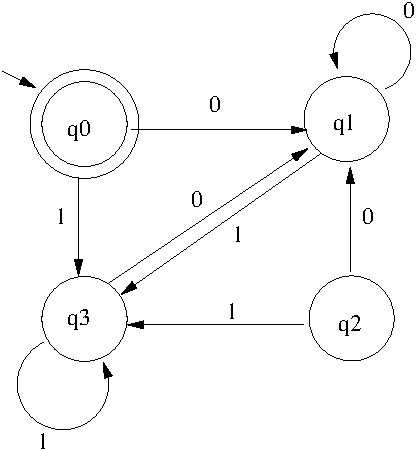
\includegraphics[width=8em]{fig}}
    \legend{Fonte: Os Autores}
    \label{fig:ex1}
\end{figure}

% o `[h]' abaixo é um parâmetro opcional que sugere que o LaTeX coloque a
% figura exatamente neste ponto do texto. Somente preocupe-se com esse tipo
% de formatação quando o texto estiver completamente pronto (uma frase a mais
% pode fazer o LaTeX mudar completamente de idéia sobre onde colocar as
% figuras e tabelas)
%\begin{figure}[h]
\begin{figure}
    \caption{Exemplo de figura desenhada com o environment \texttt{picture}.}
    \begin{center}
        \setlength{\unitlength}{.1em}
        \begin{picture}(100,100)
                \put(20,20){\circle{20}}
                \put(20,20){\small\makebox(0,0){a}}
                \put(80,80){\circle{20}}
                \put(80,80){\small\makebox(0,0){b}}
                \put(28,28){\vector(1,1){44}}
        \end{picture}
    \end{center}
    \legend{Fonte: Os Autores}
    \label{fig:ex2}
\end{figure}

Tabelas são construídas com praticamente os mesmos comandos. Ver a tabela \ref{tbl:ex1}.

\begin{table}[h]
    \caption{Uma tabela de Exemplo}
    \begin{center}
        \begin{tabular}{c|c|p{5cm}}
            \textit{Col 1}  &   \textit{Col 2}  &   \textit{Col 3} \\
            \hline
            \hline
            Val 1           &   Val 2           & Esta coluna funciona como um parágrafo, tendo uma margem definida em 5cm. Quebras de linha funcionam como em qualquer parágrafo do tex. \\
            Valor Longo     & Val 2             & Val 3 \\
            \hline
        \end{tabular}
    \end{center}
    \legend{Fonte: Os Autores}
    \label{tbl:ex1}
\end{table}

\subsection{Formato de Figuras}
\label{sec:fig_format}

O LaTeX permite utilizar vários formatos de figuras, entre eles \emph{eps}, \emph{pdf}, \emph{jpeg} e \emph{png}. Programas de diagramação como Inkscape (e mesmo LibreOffice) permitem gerar arquivos de imagens vetoriais que podem ser utilizados pelo LaTeX sem dificuldade. Pacotes externos permitem utilizar SVG e outros formatos.

Dia e xfig são programas utilizados por dinossauros para gerar figuras vetoriais. Se possível, evite-os.

\subsection{Classificação dos etc.}

O formato adotado pela ABNT prevê apenas três níveis (capítulo, seção e subseção). Assim, \texttt{\char'134subsubsection} não é aconselhado.

\section{Sobre as referências bibliográficas}

A classe \emph{iiufrgs} faz uso do pacote \emph{abnTeX2} com algumas alterações
feitas por Sandro Rama Fiorini. Culpe ele se algo der errado. Agradeça a ele
pelo que der certo. As modificações dão uma camada de tinta NATBIB-style,
já que o abntex2 usa uns comandos de citação feitos para alienígenas de 5 braços 
wtf. Exemplos de citação:

\begin{itemize}

	\item \emph{cite}: Unicórnios são verdes \cite{Nicolaidis2011};
	\item \emph{citep}:Unicórnios são verdes \citep{SimondDavidmann2014};
	\item \emph{citet}: Segundo \citet{Nicolaidis2011}, unicórnios são verdes.
	\item \emph{citen or citenum}: Segundo \citen{Rebaudengo2004}, unicórnios são verdes.
	\item \emph{citeauthor e citeyearpar}: Segundo artigos de \citeauthor{Alkhalifa1999}, unicórnios são verdes \citeyear{Nicolaidis2011}.

\end{itemize}

O estilo abnt fornecido antigamente pelo UTUG não é mais recomendado, pois não
produz saída de acordo com as exigências da biblioteca.

Recomenda-se o uso de bibtex para gerenciar as referências (veja o arquivo
biblio.bib).